\begin{figure*}[t]
\vspace*{-1.6em}
\centering
\begin{subfigure}[b]{0.5\textwidth}
  \centering
  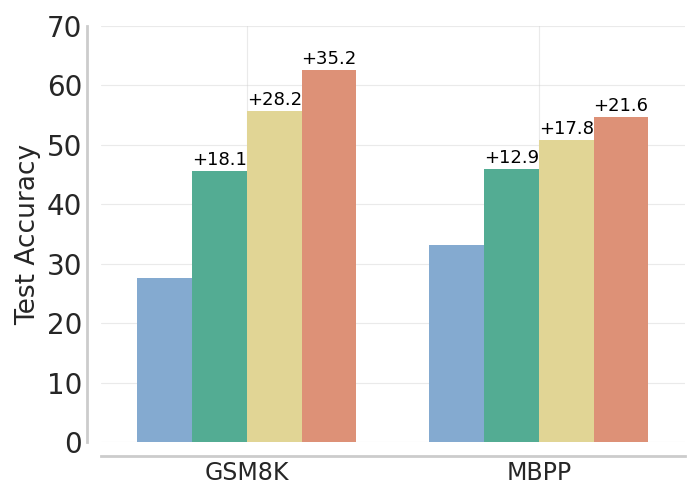
\includegraphics[scale=0.39]{icml2023/figs/benchmark_7B/bechmark_train_7B.png}
  % \caption{Tasks}
    \label{fig:main_tasks}
\end{subfigure}%
\begin{subfigure}[b]{0.5\textwidth}
  \centering
  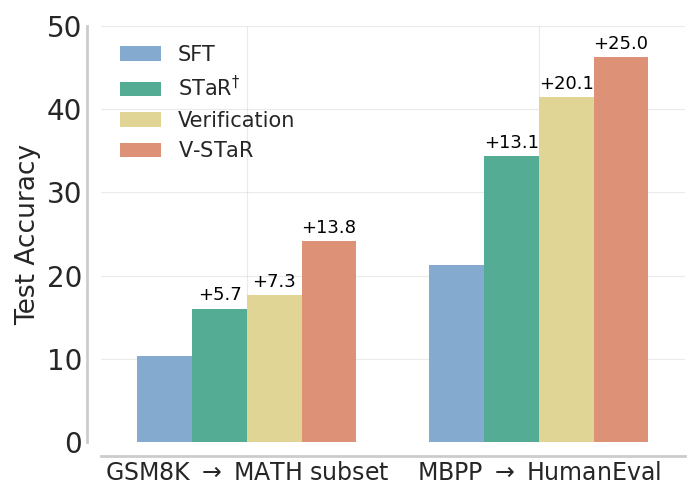
\includegraphics[scale=0.39]{icml2023/figs/benchmark_7B/bechmark_transfer_7B.png}
  % \caption{Transfer tasks}
    \label{fig:transfer_main}
\end{subfigure}%
\vspace*{-1em}
\caption{\textbf{Test accuracy of 7B \vstar{} compared to self-improvement and verification baselines.} 
We report Best-of-64 for verification-based methods and Pass$@1$ for others. All methods, except SFT, have access to the SFT baseline model and $K=48$ output generations per problem. \stardag{} and \vstar{} are run for 3 iterations, where each iteration uses $K/3 = 16$ samples. Verification corresponds to using a test-time verifier trained on K generated completions from the SFT generator. Numbers above each bar show the absolute improvement over SFT. \textbf{(Left)} Test accuracy on  tasks used for \vstar{} training. \textbf{(Right)} Transfer evaluation of GSM8K and MBPP trained models on MATH subset and HumanEval respectively.}
\label{fig:results}
\vspace{-0.1in}
\end{figure*}
